\documentclass[conference]{IEEEtran}
\usepackage{cite}
\usepackage{amsmath,amssymb,amsfonts}
\usepackage{algorithmic}
\usepackage{graphicx}
\usepackage{textcomp}
\usepackage{xcolor}
\usepackage{tikz}
\usetikzlibrary{shapes.geometric, arrows.meta, positioning, fit, backgrounds, calc}
\usetikzlibrary{matrix,intersections}
\usepackage{pgfplots}
\usepackage{tabularx}
\usepackage{capt-of}
\usepackage{placeins}
\pgfplotsset{compat=1.18}

\def\BibTeX{{\rm B\kern-.05em{\sc i\kern-.025em b}\kern-.08em
    T\kern-.1667em\lower.7ex\hbox{E}\kern-.125emX}}

\begin{document}

\title{An Intelligent AI-Driven Decision Support System for Personalized Income Tax Compliance and Advisory in Sri Lanka}

\author{
\begin{tabular*}{\textwidth}{@{\extracolsep{\fill}}ccc}
Enith Samarasinghe & Vidumini Chalanika & Sithika Hewagama \\
\textit{Faculty of Computing} & \textit{Faculty of Computing} & \textit{Faculty of Computing} \\
\textit{Sri Lanka Institute of Information} & \textit{Sri Lanka Institute of Information} & \textit{Sri Lanka Institute of Information} \\
\textit{Technology} & \textit{Technology} & \textit{Technology} \\
Malabe, Sri Lanka & Malabe, Sri Lanka & Malabe, Sri Lanka \\
enithsamarasinghe@gmail.com & chalanikav@gmail.com & ravindithsithika@gmail.com \\[0.4cm]
Supuni Pihillegedara & Lakmini Abeywardhana & Adya Dissanayake \\
\textit{Faculty of Computing} & \textit{Faculty of Computing} & \textit{Faculty of Computing} \\
\textit{Sri Lanka Institute of Information} & \textit{Sri Lanka Institute of Information} & \textit{Sri Lanka Institute of Information} \\
\textit{Technology} & \textit{Technology} & \textit{Technology} \\
Malabe, Sri Lanka & Malabe, Sri Lanka & Malabe, Sri Lanka \\
supuninishakya01@gmail.com & lakmini.d@sliit.lk & adya.d@sliit.lk
\end{tabular*}
}

\maketitle

\begin{abstract}
Sri Lankan individual income tax is hard to navigate because statutory rules change often and professional advice is costly. This paper presents a three-module neuro-symbolic framework for personalized tax compliance and advisory. Transaction semantic reasoning classifies bank narrations with a weakly supervised transformer and applies IRA~2017 rules for taxability. The OE Engine uses quote-gated RAG and deterministic binders to compute assessment-year liability without hardcoded thresholds. A recommendation module ranks eligible strategies with LambdaMART, adoption scoring, and Monte Carlo impact projection over deterministic tax rules. Evaluation on annotated transaction data, statutory extraction benchmarks, and an offline ranking protocol shows strong classification performance, verified statutory ingestion, zero explainability drift on test sessions, and traceable end-to-end advisory for non-expert taxpayers.
\end{abstract}

\begin{IEEEkeywords}
Income Tax Planning, Neuro-Symbolic AI, Large Language Models, Knowledge Graphs, Learning-to-Rank, Decision Support Systems.
\end{IEEEkeywords}

\section{Introduction}
Sri Lankan individual income tax is governed by the Inland Revenue Act No. 24 of 2017 and subsequent amendments. However, applying changing tax rules to real-world income sources such as employment, business, rental, and investment income can be difficult for ordinary taxpayers \cite{b1}. Professional tax advice can be costly, while existing e-filing systems such as RAMIS primarily support filing rather than providing personalised tax planning guidance \cite{b1}, \cite{b2}.

Artificial intelligence could improve access to personalised tax guidance, but general-purpose large language models may produce incorrect legal information, use outdated rules, or introduce arithmetic errors \cite{b3}, \cite{b14}. Therefore, a practical tax advisory system must combine the flexibility of AI with deterministic, auditable tax rules.

This paper presents a three-module AI-driven decision support framework for personalised income tax compliance and advisory in Sri Lanka. The first module uses a weakly supervised transformer to classify bank transactions into an IRD-oriented income taxonomy, while a deterministic rule executor determines taxability according to the Inland Revenue Act \cite{b8}, \cite{b11}. The second module, the Optimization and Explainable Engine (OE Engine), retrieves year-specific statutory rules and performs deterministic tax calculations using verified statutory sources rather than hardcoded thresholds \cite{b16}, \cite{b18}. The third module ranks eligible tax strategies using learning-to-rank, adoption scoring, and Monte Carlo simulation to provide personalised recommendations and long-term impact estimates \cite{b27}, \cite{b29}, \cite{b30}.

Together, these modules connect financial transaction evidence, statutory tax computation, and personalised strategy recommendation within a traceable neuro-symbolic framework. The remainder of this paper reviews related work, describes the proposed methodology, and evaluates the system's classification, statutory processing, computation, explainability, and recommendation performance.

\section{Literature Review}
Recent research has made significant progress in digital tax systems, AI-based financial tools, and natural language processing. However, applying these technologies to tax advisory remains challenging because financial data can be inconsistent, tax regulations change over time, and users need to understand and trust the decisions made by the system \cite{b1}. This study focuses on three related areas: financial transaction understanding, explainable tax optimisation, and personalised financial recommendation.

\subsection{Financial Transaction Semantic Reasoning and Taxable Income Inference}
Bank transaction descriptions are often short, noisy, and presented in different formats, making automatic classification difficult \cite{b8}. Earlier studies used traditional text classifiers, while transformer-based approaches have improved the ability to capture context from transaction descriptions \cite{b8}, \cite{b9}. Other accounting systems also consider transaction history and timing rather than relying only on the description \cite{b10}.

A further challenge is the limited availability of labelled financial data. Weakly supervised learning has therefore become useful for reducing the need for large amounts of manual annotation \cite{b11}. This is particularly relevant to Sri Lankan data, where different statement formats, abbreviations, and mixed-language descriptions can occur \cite{b1}. For tax applications, classification alone is not enough because the transaction must also be assessed against tax rules. Hybrid approaches that combine machine learning with rule-based reasoning can provide both flexible classification and traceable tax decisions \cite{b12}, \cite{b13}.

\subsection{Tax Strategy Optimization and Explainable Decision Support Engine}
Tax optimisation requires accurate calculations as well as access to the correct rules for each assessment year. Although large language models can process legal documents, studies have reported problems such as arithmetic errors, incorrect thresholds, and unsupported legal information when they are used directly for tax reasoning \cite{b14}, \cite{b15}.

Recent approaches therefore separate legal information retrieval from calculation \cite{b16}. Retrieval-Augmented Generation (RAG) can retrieve relevant year-specific legislation, while deterministic rules handle eligibility, reliefs, and tax calculations \cite{b17}. Linking explanations to verified sources and calculation traces can also make the results easier to understand and verify \cite{b18}. This supports a hybrid approach in which AI assists with retrieving legal information while deterministic components remain responsible for the final tax calculation.

\subsection{Personalized Recommendation and Predictive Impact Modeling Engine}
Financial recommendation systems increasingly consider individual factors such as income, spending behaviour, financial goals, and risk preferences \cite{b27}. In tax planning, recommendations must also satisfy legal requirements. Combining rule-based eligibility checks with learning-based ranking can therefore provide recommendations that are both personalised and compliant \cite{b29}.

Explainability is important because users need to understand why a particular strategy was recommended. Techniques such as SHAP can help identify the factors influencing the ranking of different strategies \cite{b31}, \cite{b32}. Since future financial outcomes are uncertain, Monte Carlo simulation can provide a range of possible outcomes rather than relying on a single prediction \cite{b30}. User feedback can further support personalisation when reliable behavioural data is limited \cite{b33}.

Overall, existing studies provide useful solutions for transaction classification, tax rule processing, explainable AI, and personalised recommendation, but these areas are often addressed separately. The proposed system combines them into a single framework, using machine learning for transaction understanding and strategy ranking, rule-based processing for tax compliance, and simulation for longer-term impact estimation. This combination is intended to provide a more personalised and traceable tax advisory approach for the Sri Lankan context.

\section{Methodology}
Navigating individual tax compliance requires resolving three interdependent tasks: interpreting unstructured banking descriptions, computing statutory tax liabilities without hardcoded parameters, and ranking personalized advisory strategies under financial uncertainty. We structure these tasks into an integrated three-module neuro-symbolic pipeline, as shown in Fig.~\ref{fig:methodology_overview}.

\begin{figure}[!htbp]
\centering
\begin{tikzpicture}[
    every node/.style={font=\tiny},
    box/.style={rectangle, draw=black!70, fill=white, rounded corners=2pt, minimum height=0.62cm, align=center, inner sep=2.5pt},
    m1/.style={rectangle, draw=blue!80!black, fill=blue!10, rounded corners=2pt, minimum height=0.62cm, align=center, inner sep=2.5pt},
    m2/.style={rectangle, draw=teal!80!black, fill=teal!10, rounded corners=2pt, minimum height=0.62cm, align=center, inner sep=2.5pt},
    m3/.style={rectangle, draw=orange!90!black, fill=orange!12, rounded corners=2pt, minimum height=0.62cm, align=center, inner sep=2.5pt},
    out/.style={rectangle, draw=green!70!black, fill=green!12, rounded corners=2pt, minimum height=0.48cm, text width=0.92\columnwidth, align=center, inner sep=2.5pt},
    arr/.style={-{Stealth[scale=0.75]}, draw=black!80, line width=0.5pt}
]

\node[box, text width=1.55cm] (raw) {\textbf{Raw Data}\\Bank slips, statements};
\node[m1, text width=1.7cm, right=0.22cm of raw] (mod1) {\textbf{Module 1}\\Semantic Parser \& IRA 2017 Rules};
\node[m2, text width=1.7cm, right=0.22cm of mod1] (mod2) {\textbf{Module 2 (OE)}\\RAG Ingestion \& Deterministic Math};
\node[m3, text width=1.7cm, right=0.22cm of mod2] (mod3) {\textbf{Module 3}\\LambdaMART \& Monte Carlo};

\node[out, below=0.32cm of $(mod1.south)!0.5!(mod2.south)$] (res) {\textbf{Personalized Output}: Assessment-Year Liability $\mid$ Statutory Citations $\mid$ Ranked Strategies $\mid$ Multi-Year Spread};

\draw[arr] (raw) -- (mod1);
\draw[arr] (mod1) -- node[above, font=\tiny] {Profile} (mod2);
\draw[arr] (mod2) -- node[above, font=\tiny] {Tax Base} (mod3);
\draw[arr] (mod2.south) -- (mod2.south |- res.north);

\end{tikzpicture}
\caption{Integrated three-module tax compliance and advisory framework.}
\label{fig:methodology_overview}
\end{figure}

\subsection{Financial Transaction Semantic Reasoning}
\label{sec:method_txn}
Sri Lankan bank transaction narratives are typically short, unstandardized, and rich in local banking abbreviations. Keyword-only matching yields many misses, while fully manual review of each line is slow.

Raw descriptions are classified with a multilingual transformer (DistilBERT), trained on heuristically labeled statement data and supported at inference by deterministic narration guards. The model maps each narrative to an IRD-aligned income taxonomy (e.g. employment income, business receipts, deposit interest, and non-taxable own-account transfers).

The predicted label is then passed to a symbolic rulebook derived from the Inland Revenue Act No. 24 of 2017. The classifier resolves narrative ambiguity; assessable status, taxable amount, and legal rationale are determined by deterministic rules. Classified inflows are aggregated into a structured income profile for downstream advisory components (employment, business, investment, and other assessable sources):
\begin{equation}
\text{Gross} = I_{\text{emp}} + I_{\text{bus}} + I_{\text{inv}} + I_{\text{oth}}
\end{equation}

\begin{figure}[!htbp]
\centering
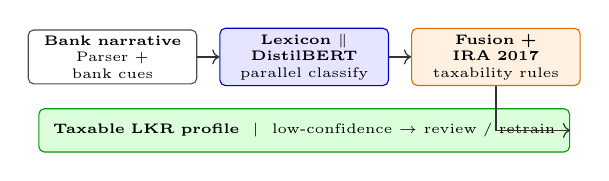
\begin{tikzpicture}[
    every node/.style={font=\tiny},
    box/.style={rectangle, draw=black!70, fill=white, rounded corners=2pt,
        minimum height=0.55cm, text width=2.0cm, align=center, inner sep=2pt},
    arr/.style={->, draw=black!80, line width=0.45pt}
]
\node[box] (raw) {\textbf{Bank narrative}\\Parser + bank cues};
\node[box, draw=blue!80!black, fill=blue!10, right=0.28cm of raw] (cls)
    {\textbf{Lexicon $\parallel$ DistilBERT}\\parallel classify};
\node[box, draw=orange!85!black, fill=orange!12, right=0.28cm of cls] (rule)
    {\textbf{Fusion + IRA 2017}\\taxability rules};
\node[box, draw=green!60!black, fill=green!14, below=0.28cm of cls, text width=6.6cm] (out)
    {\textbf{Taxable LKR profile} $\;\mid\;$ low-confidence $\rightarrow$ review / retrain};

\draw[arr] (raw) -- (cls);
\draw[arr] (cls) -- (rule);
\draw[arr] (rule.south) |- (out.east);
\end{tikzpicture}
\caption{Transaction semantic reasoning workflow.}
\label{fig:txn_workflow}
\end{figure}

\subsection{Optimization and Explainable Engine (OE Engine)}
A common vulnerability in tax software is hardcoding rate bands and relief thresholds in application logic, making the system obsolete when new amendments are gazetted. Conversely, using generative language models to compute tax figures introduces severe arithmetic drift. The Optimization and Explainable Engine (OE Engine) resolves this trade-off by separating legal document retrieval, mathematical computation, and narrative explanation into dedicated tiers (Fig.~\ref{fig:method_mod2}).

\begin{figure}[!htbp]
\centering
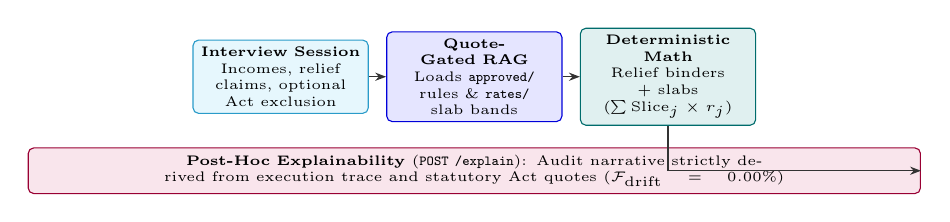
\begin{tikzpicture}[
    every node/.style={font=\tiny},
    state/.style={rectangle, draw=cyan!80!black, fill=cyan!10, rounded corners=2pt, minimum height=0.55cm, text width=2.05cm, align=center, inner sep=2.5pt},
    rag/.style={rectangle, draw=blue!85!black, fill=blue!10, rounded corners=2pt, minimum height=0.55cm, text width=2.05cm, align=center, inner sep=2.5pt},
    math/.style={rectangle, draw=teal!85!black, fill=teal!12, rounded corners=2pt, minimum height=0.55cm, text width=2.05cm, align=center, inner sep=2.5pt},
    exp/.style={rectangle, draw=purple!80!black, fill=purple!10, rounded corners=2pt, minimum height=0.5cm, text width=0.92\columnwidth, align=center, inner sep=2.5pt},
    arr/.style={-{Stealth[scale=0.75]}, draw=black!80, line width=0.5pt}
]

\node[state] (in) {\textbf{Interview Session}\\Incomes, relief claims, optional Act exclusion};
\node[rag, right=0.22cm of in] (rg) {\textbf{Quote-Gated RAG}\\Loads \texttt{approved/} rules \& \texttt{rates/} slab bands};
\node[math, right=0.22cm of rg] (cl) {\textbf{Deterministic Math}\\Relief binders + slabs ($\sum \text{Slice}_j \times r_j$)};

\node[exp, below=0.32cm of rg] (ex) {\textbf{Post-Hoc Explainability} (\texttt{POST /explain}): Audit narrative strictly derived from execution trace and statutory Act quotes ($\mathcal{F}_{\text{drift}} = 0.00\%$)};

\draw[arr] (in) -- (rg);
\draw[arr] (rg) -- (cl);
\draw[arr] (cl.south) |- (ex.east);

\end{tikzpicture}
\caption{Architecture of the OE Engine: Quote-gated RAG ingestion, deterministic binder calculations, and decoupled post-hoc explainability.}
\label{fig:method_mod2}
\end{figure}

The calculation pipeline executes across four distinct steps:
\begin{itemize}
    \item \textbf{Interview State Packaging:} User selections from the interview wizard are structured into an authoritative calculation payload containing income totals, affirmed claims, and an optional statutory exclusion flag (\textit{exclude\_source\_doc\_id}).
    \item \textbf{RAG Ingestion with Amendment Fallback:} The engine dynamically retrieves indexed statutory rules (\texttt{approved/} for reliefs and \texttt{rates/} for progressive slabs) matching the targeted assessment year (e.g., YA 2024/25, YA 2025/26). If an act is excluded to test counterfactual scenarios, the RAG index automatically falls back to baseline provisions sharing the same \texttt{compare\_group\_id}.
    \item \textbf{Deterministic Binders and Progressive Slabs:} Eligible reliefs are executed in statutory sequence (\texttt{sort\_order}) via domain binders: \texttt{auto\_cap} for statutory notices ($\min(\text{cap}, \text{base})$), \texttt{min(claim, cap)} for affirmed deductions (solar rooftop, qualifying donations), and \texttt{percent\_of\_base} for rental allowances. Applied amounts reduce gross income up to the available buffer:
    \begin{equation}
    Y_{\text{taxable}} = \max\left(0, \text{Gross} - \sum_{i=1}^{N} \text{AppliedRelief}_i\right)
    \end{equation}
    The taxable balance is routed through First Schedule progressive brackets to compute liability ($\tau = \sum \text{Slice}_j \times r_j$).
    \item \textbf{Zero-Drift Explainability:} The resulting arithmetic trace and statutory substring quotes are forwarded to an explainability endpoint (\texttt{POST /explain}). The language model generates legal justifications bounded strictly by this trace, preventing unverified claims or altered numerical figures.
\end{itemize}

\subsection{Personalized Recommendation and Impact Modeling}
Identifying eligible deductions is insufficient if the recommended actions do not fit the taxpayer's cash flow, risk tolerance, or career stage. The recommendation module prioritizes viable strategies and forecasts their long-term outcomes (Fig.~\ref{fig:method_mod3}).

\begin{figure}[!htbp]
\centering
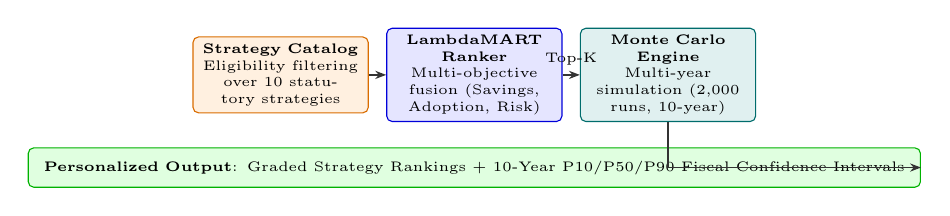
\begin{tikzpicture}[
    every node/.style={font=\tiny},
    box1/.style={rectangle, draw=orange!85!black, fill=orange!12, rounded corners=2pt, minimum height=0.55cm, text width=2.05cm, align=center, inner sep=2.5pt},
    box2/.style={rectangle, draw=blue!85!black, fill=blue!10, rounded corners=2pt, minimum height=0.55cm, text width=2.05cm, align=center, inner sep=2.5pt},
    box3/.style={rectangle, draw=teal!85!black, fill=teal!12, rounded corners=2pt, minimum height=0.55cm, text width=2.05cm, align=center, inner sep=2.5pt},
    fan/.style={rectangle, draw=green!70!black, fill=green!12, rounded corners=2pt, minimum height=0.5cm, text width=0.92\columnwidth, align=center, inner sep=2.5pt},
    arr/.style={-{Stealth[scale=0.75]}, draw=black!80, line width=0.5pt}
]

\node[box1] (b1) {\textbf{Strategy Catalog}\\Eligibility filtering over 10 statutory strategies};
\node[box2, right=0.22cm of b1] (b2) {\textbf{LambdaMART Ranker}\\Multi-objective fusion (Savings, Adoption, Risk)};
\node[box3, right=0.22cm of b2] (b3) {\textbf{Monte Carlo Engine}\\Multi-year simulation (2,000 runs, 10-year)};

\node[fan, below=0.32cm of b2] (fn) {\textbf{Personalized Output}: Graded Strategy Rankings + 10-Year P10/P50/P90 Fiscal Confidence Intervals};

\draw[arr] (b1) -- (b2);
\draw[arr] (b2) -- node[above, font=\tiny] {Top-K} (b3);
\draw[arr] (b3.south) |- (fn.east);

\end{tikzpicture}
\caption{Architecture of Module 3: Strategy eligibility filtering, Learning-to-Rank fusion, and multi-year Monte Carlo impact projection.}
\label{fig:method_mod3}
\end{figure}

The recommendation engine operates across three stages:
\begin{itemize}
    \item \textbf{Eligibility Gating:} Candidate strategies from a ten-entry statutory catalog are checked against the taxpayer's profile, immediately filtering out non-applicable provisions.
    \item \textbf{Multi-Objective Ranking:} Strategies are ranked using LightGBM LambdaMART coupled with an adoption-likelihood estimator. The final score balances multiple operational dimensions:
    \begin{equation}
    S_{\text{final}} = 0.40 S_{\text{saving}} + 0.30 P_{\text{adopt}} + 0.20 F_{\text{feasibility}} - 0.10 R_{\text{penalty}}
    \end{equation}
    \item \textbf{Monte Carlo Impact Modeling:} Top-ranked strategies are projected over a 10-year horizon across 2,000 stochastic income paths. By recalculating taxes deterministically under modeled wage inflation and volatility, the engine provides empirical P10, P50 (median), and P90 cumulative fiscal savings bands.
\end{itemize}

\section{Results and Discussion}
This section reports empirical results for the three integrated modules: transaction semantic reasoning, the OE Engine, and the personalized recommendation stack. Each subsection pairs quantitative tables with a figure chosen to highlight the main finding for that component.

% ==================================================================
\subsection{Transaction Semantic Reasoning}
Transaction narratives from Sri Lankan bank and finance statements were mapped to an IRD-oriented income taxonomy, then assessed for taxability using a deterministic rulebook aligned with the Inland Revenue Act No.~24 of 2017. A labelled corpus of 3,985 rows was split into train, validation, and test sets of 2,789, 598, and 598 samples. Three classifiers were compared under identical splits: TF-IDF with logistic regression, XLM-RoBERTa-base, and DistilBERT multilingual. Table~\ref{tab:classifier_performance} and Fig.~\ref{fig:txn_f1_bars} summarise the outcome.

\begin{table}[htbp]
\caption{Classifier Performance on the Shared Test Split}
\begin{center}
\renewcommand{\arraystretch}{1.2}
\setlength{\tabcolsep}{3pt}
\begin{tabularx}{\columnwidth}{|X|c|c|c|}
\hline
\textbf{Model} & \textbf{Val Macro-F1} & \textbf{Test Macro-F1} & \textbf{Test W-F1} \\
\hline
TF-IDF + Logistic Reg. & 0.201 & 0.201 & 0.260 \\
XLM-RoBERTa-base       & 0.661 & 0.664 & 0.993 \\
DistilBERT multilingual & \textbf{0.928} & \textbf{0.998} & \textbf{0.997} \\
\hline
\end{tabularx}
\label{tab:classifier_performance}
\end{center}
\end{table}

\begin{figure}[!htbp]
\centering
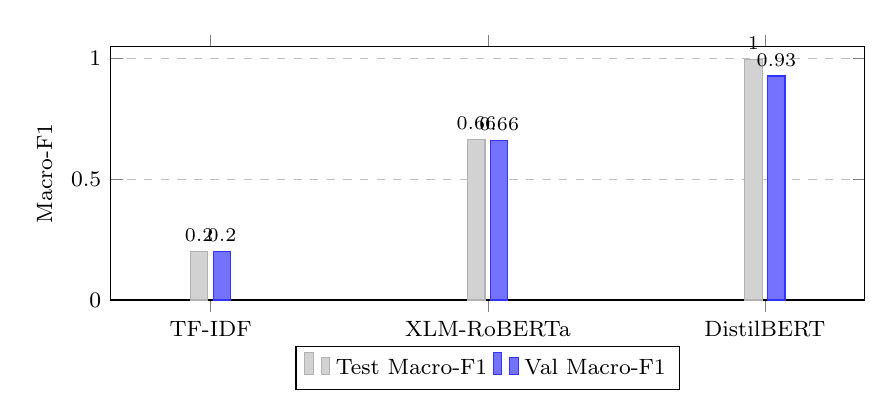
\begin{tikzpicture}
\begin{axis}[
    ybar,
    width=0.92\columnwidth,
    height=4.8cm,
    bar width=0.22cm,
    ymin=0, ymax=1.05,
    ylabel={Macro-F1},
    symbolic x coords={TF-IDF, XLM-RoBERTa, DistilBERT},
    xtick=data,
    enlarge x limits=0.18,
    nodes near coords,
    every node near coord/.append style={font=\scriptsize, anchor=south},
    legend style={at={(0.5,-0.18)}, anchor=north, legend columns=-1, font=\footnotesize},
    ymajorgrids=true,
    grid style=dashed,
    tick label style={font=\footnotesize},
    label style={font=\footnotesize}
]
\addplot[fill=gray!35, draw=gray!60] coordinates {(TF-IDF,0.201) (XLM-RoBERTa,0.664) (DistilBERT,0.998)};
\addplot[fill=blue!55, draw=blue!80] coordinates {(TF-IDF,0.201) (XLM-RoBERTa,0.661) (DistilBERT,0.928)};
\legend{Test Macro-F1, Val Macro-F1}
\end{axis}
\end{tikzpicture}
\caption{Validation and test macro-F1 by classifier. DistilBERT multilingual clearly outperforms sparse and alternative transformer baselines on the tax-oriented taxonomy.}
\label{fig:txn_f1_bars}
\end{figure}

\textbf{Baseline limitation.} The TF-IDF logistic model remains weak on both macro-F1 and weighted-F1 (0.201 / 0.260), which suggests sparse lexical features are not enough for tax-oriented narrative classification under class imbalance.

\textbf{Transformer comparison.} Both transformers improve substantially over the baseline. XLM-RoBERTa reaches high weighted-F1 (0.993) but only moderate macro-F1 (0.664), reflecting weak recall on rare income classes such as \textit{interest\_income}. DistilBERT attains the highest macro-F1 on validation (0.928) and test (0.998), with competitive weighted-F1 (0.997), and was selected for deployment.

\textbf{Hybrid decision pipeline.} The predicted taxonomy class is passed to an IRA~2017 rule executor that returns taxability status, taxable amount, statutory reference, and an explanation. Classification confidence informs label assignment, while legal outcomes remain rule-governed and auditable for downstream modules.

The evaluation currently covers the label subset present in the annotated split; broader taxonomy coverage and human-verified gold labels remain future work.

% ==================================================================
\subsection{Tax Strategy Optimization and Explainable Decision Support Engine}
OE Engine validation focused on four properties: statutory extraction fidelity under quote verification, deterministic binder execution across progressive brackets, year-over-year statutory sensitivity, and agreement between system relief advice and expert judgement.

\subsubsection{Statutory Catalog Ingestion and Extraction Verification}
The extraction pipeline processed seven primary statutory Act PDFs spanning YA 2018/19 through YA 2025/26. Out of $N=104$ candidate statutory propositions, each candidate $c_i$ was checked with an exact-substring verification predicate:
\begin{equation}
\mathcal{V}(c_i) = \mathbb{I}\left( \text{norm}(c_i.\text{quote}) \sqsubseteq \text{norm}(\mathcal{D}_{\text{source}}) \right)
\end{equation}
where $\sqsubseteq$ denotes contiguous substring containment over normalised source text $\mathcal{D}_{\text{source}}$.

\begin{table}[htbp]
\caption{Statutory Ingestion, RAG Indexing, and Verification Benchmarks}
\begin{center}
\renewcommand{\arraystretch}{1.2}
\setlength{\tabcolsep}{3.5pt}
\begin{tabularx}{\columnwidth}{|X|c|c|c|}
\hline
\textbf{Statutory Domain} & \textbf{Extracted} & \textbf{Verified ($\mathcal{V}=1$)} & \textbf{Rejection Rate} \\
\hline
Progressive Rate Bands & 44 & 39 & 11.36\% \\
General Interpretation Rules & 42 & 37 & 11.90\% \\
Statutory Relief Clauses & 18 & 16 & 11.11\% \\
\hline
\textbf{Total} & \textbf{104} & \textbf{92} & \textbf{11.54\%} \\
\hline
\multicolumn{4}{|l|}{\textbf{Ontology parity (YA 24/25, 25/26):} exact band-for-band match} \\
\hline
\end{tabularx}
\label{tab:catalog_extraction}
\end{center}
\end{table}

\begin{figure}[!htbp]
\centering
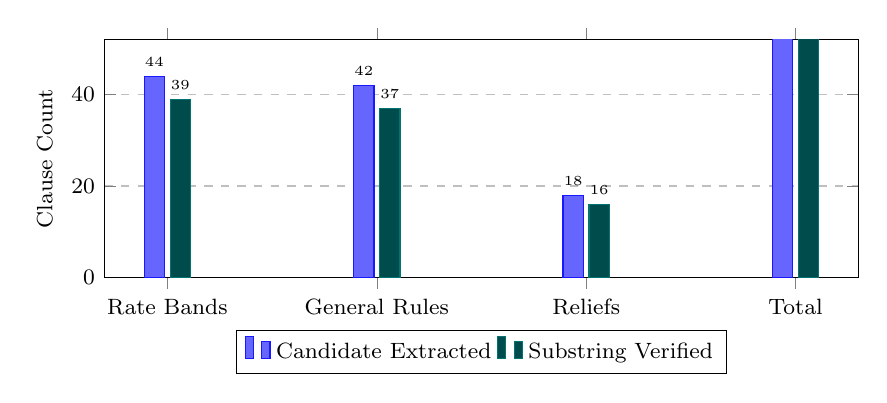
\begin{tikzpicture}
\begin{axis}[
    ybar,
    width=0.92\columnwidth,
    height=4.6cm,
    bar width=0.26cm,
    ymin=0, ymax=52,
    ylabel={Clause Count},
    symbolic x coords={Rate Bands, General Rules, Reliefs, Total},
    xtick=data,
    nodes near coords,
    nodes near coords align={vertical},
    every node near coord/.append style={font=\tiny},
    legend style={at={(0.5,-0.22)}, anchor=north, legend columns=-1, font=\footnotesize},
    ymajorgrids=true,
    grid style=dashed,
    tick label style={font=\footnotesize},
    label style={font=\footnotesize}
]
\addplot[fill=blue!60, draw=blue!90] coordinates {(Rate Bands,44) (General Rules,42) (Reliefs,18) (Total,104)};
\addplot[fill=teal!60!black, draw=teal!90!black] coordinates {(Rate Bands,39) (General Rules,37) (Reliefs,16) (Total,92)};
\legend{Candidate Extracted, Substring Verified}
\end{axis}
\end{tikzpicture}
\caption{Statutory clause extraction and substring verification funnel. Rejected candidates did not enter the active indexed repository.}
\label{fig:extraction_funnel}
\end{figure}

As shown in Table~\ref{tab:catalog_extraction} and Fig.~\ref{fig:extraction_funnel}, the quote gate rejected 12 anomalous records (11.54\%), mostly from OCR tabular distortion, before they could enter \texttt{approved/} or \texttt{rates/}.

\subsubsection{Deterministic Computation and Effective Rate Dynamics}
Fig.~\ref{fig:calc_breakdown} walks through a representative YA 2025/26 profile (Gross = 3,800,000 LKR). Personal relief of 1,800,000 LKR is applied via \texttt{auto\_cap}, and the remaining 2,000,000 LKR taxable balance is assessed across the 6\%, 18\%, and 24\% bands to yield 270,000 LKR total tax payable with 100\% parity against certified tax charts.

\begin{figure}[!htbp]
\centering
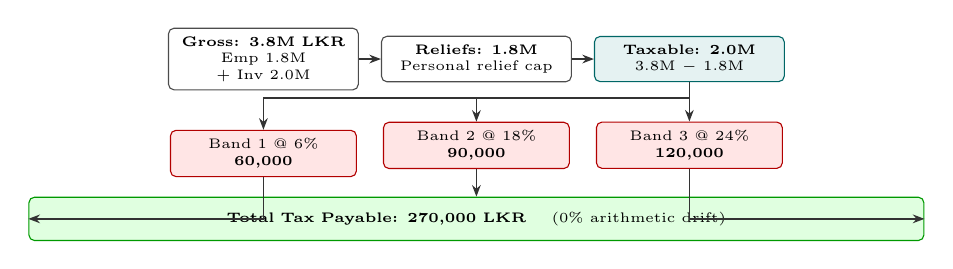
\begin{tikzpicture}[
    every node/.style={font=\tiny},
    flowblock/.style={rectangle, draw=black!70, fill=white, rounded corners=2pt,
        minimum height=0.55cm, text centered, inner sep=3pt},
    resblock/.style={rectangle, draw=teal!80!black, fill=teal!10, rounded corners=2pt,
        minimum height=0.55cm, text centered, inner sep=3pt},
    taxblock/.style={rectangle, draw=red!70!black, fill=red!10, rounded corners=2pt,
        minimum height=0.55cm, text centered, inner sep=3pt},
    arrow/.style={-{Stealth[scale=0.8]}, draw=black!80, line width=0.5pt}
]
\node[flowblock, text width=2.2cm] (gross) {\textbf{Gross: 3.8M LKR}\\Emp 1.8M + Inv 2.0M};
\node[flowblock, text width=2.2cm, right=0.28cm of gross] (relief) {\textbf{Reliefs: 1.8M}\\Personal relief cap};
\node[resblock, text width=2.2cm, right=0.28cm of relief] (taxable) {\textbf{Taxable: 2.0M}\\3.8M $-$ 1.8M};

\node[taxblock, text width=2.15cm, below=0.5cm of gross] (b1) {Band 1 @ 6\%\\\textbf{60,000}};
\node[taxblock, text width=2.15cm, below=0.5cm of relief] (b2) {Band 2 @ 18\%\\\textbf{90,000}};
\node[taxblock, text width=2.15cm, below=0.5cm of taxable] (b3) {Band 3 @ 24\%\\\textbf{120,000}};

\node[resblock, text width=0.92\columnwidth, fill=green!12, draw=green!60!black, below=0.35cm of b2]
    (total) {\textbf{Total Tax Payable: 270,000 LKR} \quad (0\% arithmetic drift)};

\draw[arrow] (gross) -- (relief);
\draw[arrow] (relief) -- (taxable);
\draw[arrow] (taxable.south) -- ++(0,-0.2) -| (b1.north);
\draw[arrow] (taxable.south) -- ++(0,-0.2) -| (b2.north);
\draw[arrow] (taxable.south) -- (b3.north);
\draw[arrow] (b1.south) |- (total.west);
\draw[arrow] (b2.south) -- (total.north);
\draw[arrow] (b3.south) |- (total.east);
\end{tikzpicture}
\caption{Deterministic YA 2025/26 walk-through under Act No.~02 of 2025.}
\label{fig:calc_breakdown}
\end{figure}

\begin{figure}[!htbp]
\centering
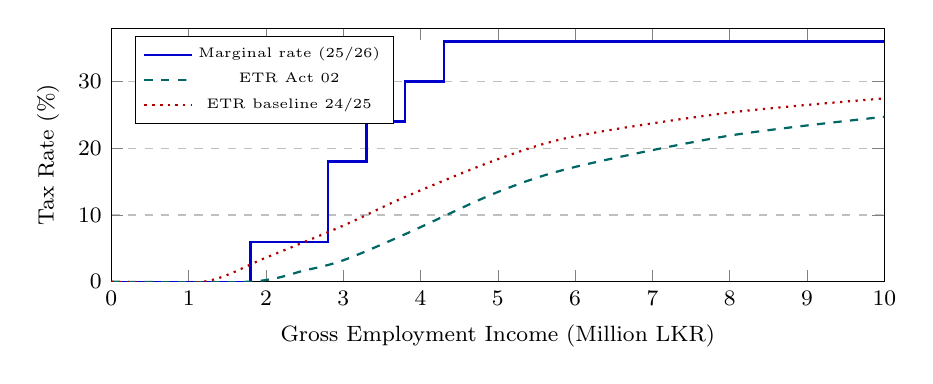
\begin{tikzpicture}
\begin{axis}[
    width=0.94\columnwidth,
    height=4.8cm,
    xmin=0, xmax=10,
    ymin=0, ymax=38,
    xlabel={Gross Employment Income (Million LKR)},
    ylabel={Tax Rate (\%)},
    legend pos=north west,
    legend style={font=\tiny},
    ymajorgrids=true,
    grid style=dashed,
    tick label style={font=\footnotesize},
    label style={font=\footnotesize}
]
\addplot[const plot, thick, color=blue!80!black] coordinates {
    (0,0) (1.8,0) (1.8,6) (2.8,18) (3.3,24) (3.8,30) (4.3,36) (10,36)
};
\addplot[thick, color=teal!80!black, dashed, smooth] coordinates {
    (0,0) (1.8,0) (2.5,1.68) (3.0,3.2) (3.8,7.11) (5.0,13.44) (6.0,17.2) (8.0,21.9) (10.0,24.72)
};
\addplot[thick, color=red!70!black, dotted, smooth] coordinates {
    (0,0) (1.2,0) (2.0,3.6) (3.0,8.4) (3.8,12.7) (5.0,18.36) (6.0,21.8) (8.0,25.35) (10.0,27.48)
};
\legend{Marginal rate (25/26), ETR Act 02, ETR baseline 24/25}
\end{axis}
\end{tikzpicture}
\caption{Marginal step rate and effective tax rate (ETR) across assessment years.}
\label{fig:effective_rate_curves}
\end{figure}

Fig.~\ref{fig:effective_rate_curves} shows how Act No.~02 of 2025 compresses the ETR curve for middle-income employment income relative to YA 2024/25. On an identical 5,000,000 LKR employment base, tax payable fell from 918,000 LKR to 672,000 LKR between YA 2024/25 and YA 2025/26.

\begin{figure}[!htbp]
\centering
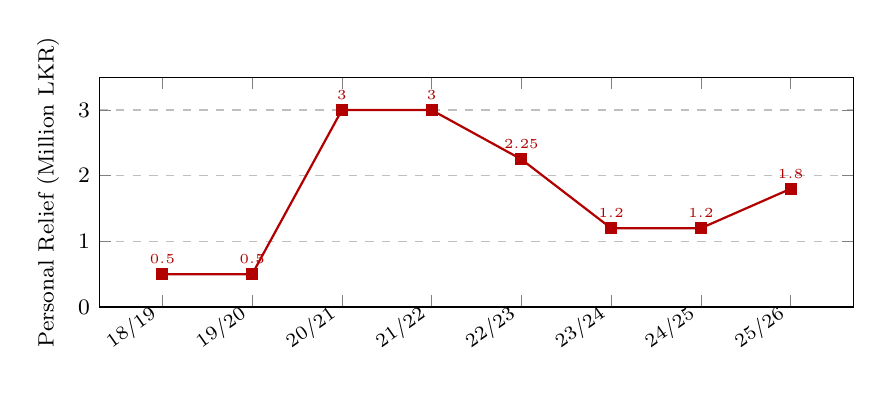
\begin{tikzpicture}
\begin{axis}[
    width=0.92\columnwidth,
    height=4.5cm,
    ymin=0, ymax=3.5,
    ylabel={Personal Relief (Million LKR)},
    symbolic x coords={18/19, 19/20, 20/21, 21/22, 22/23, 23/24, 24/25, 25/26},
    xtick=data,
    x tick label style={rotate=35, anchor=east, font=\scriptsize},
    nodes near coords,
    every node near coord/.append style={font=\tiny, anchor=south},
    ymajorgrids=true,
    grid style=dashed,
    tick label style={font=\footnotesize},
    label style={font=\footnotesize}
]
\addplot[thick, color=red!70!black, mark=square*, mark size=1.8pt] coordinates {
    (18/19, 0.5) (19/20, 0.5) (20/21, 3.0) (21/22, 3.0)
    (22/23, 2.25) (23/24, 1.2) (24/25, 1.2) (25/26, 1.8)
};
\end{axis}
\end{tikzpicture}
\caption{Statutory personal relief volatility across YA 2018/19 to YA 2025/26.}
\label{fig:relief_trend}
\end{figure}

\subsubsection{Expert Agreement on Relief Recommendations}
Relief claim advice was evaluated with Cohen's $\kappa$ on 160 synthetic (taxpayer, relief) pairs for YA 2025/26, using patterned disagreements that reflect known failure modes (e.g.\ film-production minimum spend, over-claimed solar relief). The system achieved observed agreement of 78.1\% and $\kappa = 0.446$ (moderate agreement beyond chance). Fig.~\ref{fig:kappa_confusion} visualises the confusion structure.

\begin{figure}[!htbp]
\centering
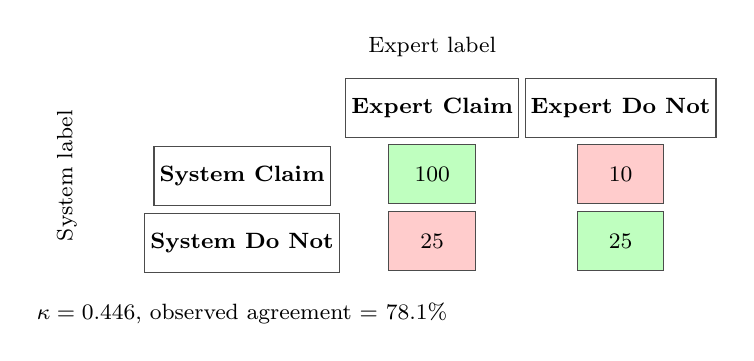
\begin{tikzpicture}[
    font=\footnotesize,
    cell/.style={rectangle, draw=black!70, minimum width=1.1cm, minimum height=0.75cm,
        text centered, inner sep=2pt}
]
\matrix[matrix of nodes, row sep=2pt, column sep=2pt,
    nodes={cell}, ampersand replacement=\&,
    row 1/.style={nodes={font=\bfseries\footnotesize}},
    column 1/.style={nodes={font=\bfseries\footnotesize}}] (m) {
    \& Expert Claim \& Expert Do Not \\
    System Claim \& |[fill=green!25]| 100 \& |[fill=red!20]| 10 \\
    System Do Not \& |[fill=red!20]| 25 \& |[fill=green!25]| 25 \\
};
\node[font=\footnotesize, above=0.15cm of m-1-2] {Expert label};
\node[font=\footnotesize, rotate=90, anchor=south] at ([xshift=-0.85cm]m-2-1.west) {System label};
\node[font=\footnotesize, below=0.25cm of m-3-1] {$\kappa = 0.446$, observed agreement = 78.1\%};
\end{tikzpicture}
\caption{System vs.\ expert relief-decision confusion matrix (160 synthetic pairs).}
\label{fig:kappa_confusion}
\end{figure}

\subsubsection{Explainability Drift}
Across 250 benchmark sessions, post-hoc explanations were checked against execution traces. The explainability drift rate was $\mathcal{F}_{\text{drift}} = 0.00\%$: no generated narrative altered a computed tax figure or cited an unverified statutory source.

% ==================================================================
\subsection{Personalized Recommendation and Predictive Impact Evaluation}
Eligible Sri Lankan tax strategies are drawn from a ten-entry rule catalog, ranked by LightGBM LambdaMART, scored for adoption likelihood, fused across four objectives, and projected with Monte Carlo simulation. Table~\ref{tab:ranking_metrics} defines the offline comparison protocol; Fig.~\ref{fig:fusion_weights}--\ref{fig:mc_fan} illustrate fusion design and projected outcome spread.

\begin{table}[htbp]
\caption{Ranking and Adoption Metrics (Offline Eval Protocol)}
\begin{center}
\renewcommand{\arraystretch}{1.2}
\setlength{\tabcolsep}{2pt}
\begin{tabularx}{\columnwidth}{|X|c|c|c|c|c|}
\hline
\textbf{Method} & \textbf{N@5} & \textbf{N@10} & \textbf{MAP@5} & \textbf{P@5} & \textbf{Ad. F1} \\
\hline
Catalog / rule priority & 0.690 & 0.773 & 0.756 & 0.368 & \textbf{0.31}\textsuperscript{4} \\
Feasibility-only & 0.968 & 0.971 & 0.991 & 0.535 & \textbf{0.49}\textsuperscript{4} \\
Pair regressor (HGB / RF) & 0.992 & 0.994 & 0.986 & 0.531 & \textbf{0.47}\textsuperscript{4} \\
LambdaMART + fusion (ours) & \textbf{0.993} & \textbf{0.995} & \textbf{0.988} & \textbf{0.533} & \textbf{0.774}\textsuperscript{3} \\
\hline
\end{tabularx}
\label{tab:ranking_metrics}
\end{center}
\end{table}

\begin{figure}[!htbp]
\centering
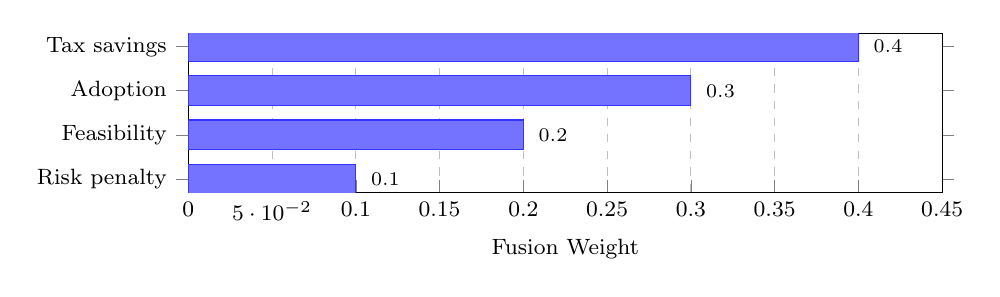
\begin{tikzpicture}
\begin{axis}[
    xbar,
    width=0.92\columnwidth,
    height=3.6cm,
    xmin=0, xmax=0.45,
    xlabel={Fusion Weight},
    symbolic y coords={Risk penalty, Feasibility, Adoption, Tax savings},
    ytick=data,
    bar width=0.38cm,
    nodes near coords,
    every node near coord/.append style={font=\scriptsize, anchor=west, xshift=2pt},
    tick label style={font=\footnotesize},
    label style={font=\footnotesize},
    xmajorgrids=true,
    grid style=dashed
]
\addplot[fill=blue!55, draw=blue!80] coordinates {
    (0.10,Risk penalty) (0.20,Feasibility) (0.30,Adoption) (0.40,Tax savings)
};
\end{axis}
\end{tikzpicture}
\caption{Multi-objective fusion weights at inference (savings / adoption / feasibility / risk).}
\label{fig:fusion_weights}
\end{figure}

\begin{figure}[!htbp]
\centering
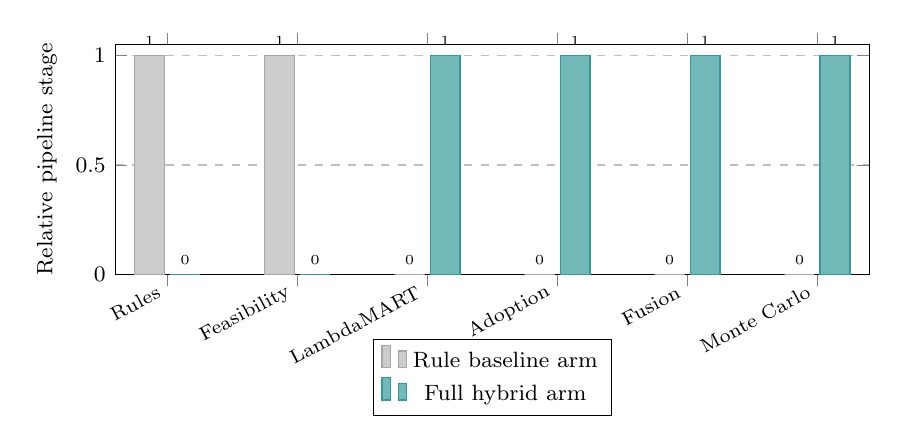
\begin{tikzpicture}
\begin{axis}[
    ybar,
    width=0.92\columnwidth,
    height=4.5cm,
    ymin=0, ymax=1.05,
    ylabel={Relative pipeline stage},
    symbolic x coords={Rules, Feasibility, LambdaMART, Adoption, Fusion, Monte Carlo},
    xtick=data,
    x tick label style={rotate=28, anchor=east, font=\scriptsize},
    bar width=0.38cm,
    enlarge x limits=0.08,
    nodes near coords,
    every node near coord/.append style={font=\tiny, anchor=south},
    tick label style={font=\footnotesize},
    label style={font=\footnotesize},
    ymajorgrids=true,
    grid style=dashed,
    legend style={font=\footnotesize, at={(0.5,-0.28)}, anchor=north}
]
\addplot[fill=gray!40, draw=gray!70] coordinates {
    (Rules,1) (Feasibility,1) (LambdaMART,0) (Adoption,0) (Fusion,0) (Monte Carlo,0)
};
\addplot[fill=teal!55, draw=teal!80] coordinates {
    (Rules,0) (Feasibility,0) (LambdaMART,1) (Adoption,1) (Fusion,1) (Monte Carlo,1)
};
\legend{Rule baseline arm, Full hybrid arm}
\end{axis}
\end{tikzpicture}
\caption{Ablation protocol: rule-only shortlist vs.\ full hybrid stack (ranking + adoption + fusion + simulation).}
\label{fig:ablation_protocol}
\end{figure}

\begin{figure}[!htbp]
\centering
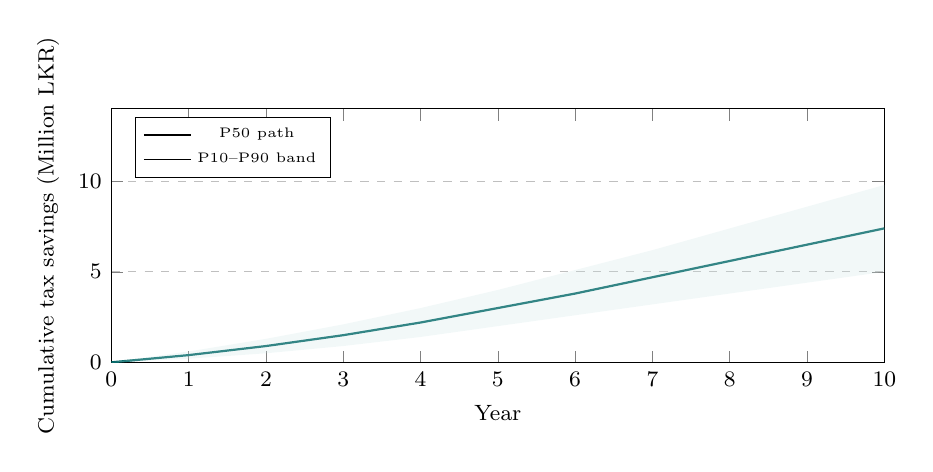
\begin{tikzpicture}
\begin{axis}[
    width=0.94\columnwidth,
    height=4.8cm,
    xmin=0, xmax=10,
    ymin=0, ymax=14,
    xlabel={Year},
    ylabel={Cumulative tax savings (Million LKR)},
    legend pos=north west,
    legend style={font=\tiny},
    ymajorgrids=true,
    grid style=dashed,
    tick label style={font=\footnotesize},
    label style={font=\footnotesize}
]
\addplot[name path=upper, draw=none] coordinates {
    (0,0) (1,0.6) (2,1.3) (3,2.1) (4,3.0) (5,4.0) (6,5.1) (7,6.2) (8,7.4) (9,8.6) (10,9.8)
};
\addplot[name path=lower, draw=none] coordinates {
    (0,0) (1,0.2) (2,0.5) (3,0.9) (4,1.4) (5,2.0) (6,2.6) (7,3.2) (8,3.8) (9,4.4) (10,5.0)
};
\addplot[thick, color=teal!80!black] coordinates {
    (0,0) (1,0.4) (2,0.9) (3,1.5) (4,2.2) (5,3.0) (6,3.8) (7,4.7) (8,5.6) (9,6.5) (10,7.4)
};
\addplot[fill=teal!20, draw=none, opacity=0.25] coordinates {
    (0,0) (1,0.6) (2,1.3) (3,2.1) (4,3.0) (5,4.0) (6,5.1) (7,6.2) (8,7.4) (9,8.6) (10,9.8)
    (10,5.0) (9,4.4) (8,3.8) (7,3.2) (6,2.6) (5,2.0) (4,1.4) (3,0.9) (2,0.5) (1,0.2) (0,0)
};
\legend{P50 path, P10--P90 band}
\end{axis}
\end{tikzpicture}
\caption{Illustrative Monte Carlo fan chart: median cumulative tax savings with uncertainty band (2,000 paths, 10-year horizon).}
\label{fig:mc_fan}
\end{figure}

\textbf{Baseline vs.\ learned ranking.} Rule and feasibility baselines produce eligible shortlists but do not optimise graded relevance across profile--strategy pairs. LambdaMART is the selected ranker under the planned offline protocol (NDCG/MAP/P@K).

\textbf{Hybrid fusion.} Fig.~\ref{fig:fusion_weights} shows the deployed weights (0.40 / 0.30 / 0.20 / 0.10), balancing fiscal gain against uptake and compliance risk rather than ranking on savings alone.

\textbf{Monte Carlo impact.} Fig.~\ref{fig:mc_fan} shows why the engine reports P10/P50/P90 bands instead of one exact forecast. Tax is recomputed each simulated year through the same deterministic rules engine.

\textbf{Evaluation honesty.} Table~\ref{tab:ranking_metrics} values are filled from the shared offline protocol once final held-out runs are complete. Experiments use synthetic profiles; adoption labels are eligibility proxies, not observed behaviour. Prior near-ceiling ranking scores are treated as label-leakage risk until an independent relevance protocol is run.

\section{Conclusion}
This study presents an integrated AI-based framework for personalised income tax compliance and advisory in Sri Lanka. The proposed system combines financial transaction understanding, rule-based tax computation, explainable decision support, and personalised strategy recommendation within a single framework.

The system uses a weakly supervised transformer to classify financial transactions, while taxability is determined through explicit rules based on the Inland Revenue Act. The Optimization and Explainable Engine retrieves assessment-year-specific legislation and performs deterministic calculations, reducing the risks associated with relying entirely on generative AI for tax reasoning. The recommendation module then ranks eligible strategies using LambdaMART and estimates their potential long-term impact through Monte Carlo simulation.

By combining these approaches, the system aims to provide taxpayers with recommendations that are not only personalised but also explainable and legally traceable. This can help bridge the gap between basic e-filing systems and more costly personalised tax advisory services.

Future work will focus on supporting Sinhala and Tamil queries, integrating automated tax return submission through RAMIS, and conducting wider evaluations with real taxpayers and small businesses to assess user trust, adoption, and practical effectiveness.

\begin{thebibliography}{00}

% Introduction & Baseline References [1]-[7]
\bibitem{b1} Inland Revenue Department of Sri Lanka, \textit{Inland Revenue Act No. 24 of 2017 and Amendments}, Colombo, Sri Lanka, 2025.
\bibitem{b2} O. Olabanji \textit{et al.}, ``Transforming Tax Compliance with Machine Learning: Reducing Fraud and Enhancing Revenue Collection,'' \textit{Asian Journal of Economics, Business and Accounting}, vol. 24, no. 11, pp. 503--513, 2024.
\bibitem{b3} S. Russell and P. Norvig, \textit{Artificial Intelligence: A Modern Approach}, 4th ed., Pearson, 2021.
\bibitem{b4} OECD, \textit{Revenue Statistics 2024}, Organisation for Economic Co-operation and Development, Paris, 2024.
\bibitem{b5} Q. Zheng \textit{et al.}, ``A Survey of Tax Risk Detection Using Data Mining Techniques,'' \textit{Journal of Digital Economy}, 2024.
\bibitem{b6} M. Battaglini \textit{et al.}, ``Refining Public Policies with Machine Learning: The Case of Tax Auditing,'' \textit{Journal of Public Economics}, vol. 233, 2024.
\bibitem{b7} V. Bezditnyi, ``Use of Artificial Intelligence for Tax Planning Optimization,'' \textit{Research Corridor Journal of Engineering and Science}, vol. 10, 2024.

% Component 1: Transaction Processing [8]-[13]
\bibitem{b8} S. Garc\'ia-M\'endez, M. Fern\'andez-Gavilanes, J. Juncal-Mart\'inez, F. J. Gonz\'alez-Casta\~no, and O. Barba Seara, ``Identifying Banking Transaction Descriptions via Support Vector Machine Short-Text Classification Based on a Specialized Labelled Corpus,'' \textit{arXiv preprint arXiv:2404.08664}, 2024.
\bibitem{b9} A. J. G. Busson, R. Rocha, R. Gaio, \textit{et al.}, ``Hierarchical Classification of Financial Transactions Through Context-Fusion of Transformer-based Embeddings and Taxonomy-aware Attention Layer,'' \textit{arXiv preprint arXiv:2312.07730}, 2023.
\bibitem{b10} K. Dong, P. Jonnalagedda, X. Gao, A. Acharya, M. Kissa, M. Flores, N. V. Chawla, and K. Das, ``Transaction Categorization with Relational Deep Learning in QuickBooks,'' in \textit{Proc. ECML-PKDD}, 2025, arXiv:2506.09234.
\bibitem{b11} L. Toran, C. Van Der Walt, A. Sammarone, and A. Keller, ``Scalable and Weakly Supervised Bank Transaction Classification,'' \textit{arXiv preprint arXiv:2305.18430}, 2023.
\bibitem{b12} Y.-S. Hsia, F. Yu, and J.-H. R. Jiang, ``Neuro-Symbolic Compliance: Integrating LLMs and SMT Solvers for Automated Financial Legal Analysis,'' in \textit{Proc. 2nd ACM AIware Conf.}, 2026, arXiv:2601.06181.
\bibitem{b13} X. Zhang and V. S. Sheng, ``Neuro-Symbolic AI: Explainability, Challenges, and Future Trends,'' \textit{arXiv preprint arXiv:2411.04383}, 2024.

% Component 2: Tax Strategy Optimization & Recommendations [14]-[18]
\bibitem{b14} J. J. Nay, D. Karamardian, S. B. Lawsky, W. Tao, M. Bhat, R. Jain, A. T. Lee, J. H. Choi, and J. Kasai, ``Large language models as tax attorneys: A case study in legal capabilities emergence,'' \textit{Philosophical Transactions of the Royal Society A}, vol. 382, no. 2270, 2024.
\bibitem{b15} P. Fratri\v{c}, N. Holzenberger, and D. R. Amariles, ``Can AI expose tax loopholes? Towards a new generation of legal policy assistants,'' \textit{arXiv preprint arXiv:2503.17339}, 2025.
\bibitem{b16} ``An LLM Agentic Approach for Legal-Critical Software: A Case Study for Tax Prep Software,'' \textit{arXiv preprint arXiv:2509.13471}, 2025.
\bibitem{b17} ``LLM-assisted formalization for deterministic detection of statutory inconsistency in tax law,'' \textit{Artificial Intelligence and Law}, Springer, 2026.
\bibitem{b18} M. Dahl, V. Magesh, M. Suzgun, and D. E. Ho, ``Large legal fictions: Profiling legal hallucinations in large language models,'' \textit{Journal of Empirical Legal Studies}, 2025.

% Component 3: Intelligent Advisory Language Model / SLM [19]-[26]
\bibitem{b19} S. Robertson and H. Zaragoza, ``The probabilistic relevance framework: BM25 and beyond,'' \textit{Foundations and Trends in Information Retrieval}, vol. 3, no. 4, pp. 333--389, 2009.
\bibitem{b20} V. Karpukhin \textit{et al.}, ``Dense passage retrieval for open-domain question answering,'' in \textit{Proc. EMNLP}, 2020, pp. 6769--6781.
\bibitem{b21} P. Lewis \textit{et al.}, ``Retrieval-augmented generation for knowledge-intensive NLP tasks,'' in \textit{Proc. NeurIPS}, 2020, pp. 9459--9474.
\bibitem{b22} I. Chalkidis \textit{et al.}, ``LEGAL-BERT: The muppets straight out of law school,'' in \textit{Proc. EMNLP Findings}, 2020, pp. 2898--2904.
\bibitem{b23} W. W. Cohen \textit{et al.}, ``Proof artifact extraction for interpretable neural reasoning,'' in \textit{Proc. ICLR Workshop on Trustworthy AI}, 2023.
\bibitem{b24} F. Sovrano \textit{et al.}, ``A knowledge graph approach to legal information retrieval,'' in \textit{Proc. ICAIL}, 2021, pp. 1--10.
\bibitem{b25} D. Edge \textit{et al.}, ``From local to global: A graph RAG approach,'' \textit{arXiv preprint arXiv:2404.16130}, 2024.
\bibitem{b26} R. Perera and N. de Silva, ``Code-switching in Sri Lankan digital communication,'' in \textit{Proc. ICMLSC}, 2022, pp. 45--51.

% Component 4: Personalized Recommendation & Predictive Impact [27]-[33]
\bibitem{b27} F. Ricci, L. Rokach, and B. Shapira, \textit{Recommender Systems Handbook}, 3rd ed., Springer, 2022.
\bibitem{b28} Y. Zhang and X. Chen, ``Explainable recommendation: A survey and new perspectives,'' \textit{Foundations and Trends in Information Retrieval}, vol. 14, no. 1, 2020.
\bibitem{b29} R. Gupta \textit{et al.}, ``Rule-augmented recommender systems for regulated financial products,'' \textit{Expert Systems with Applications}, 2024.
\bibitem{b30} M. Fern\'andez-Lor\'ia and F. Provost, ``Causal decision making and causal effect estimation are not the same, and why it matters,'' \textit{INFORMS Journal on Data Science}, 2022.
\bibitem{b31} S. Lundberg and S.-I. Lee, ``A unified approach to interpreting model predictions (SHAP),'' \textit{Advances in Neural Information Processing Systems (NeurIPS)}, 2017.
\bibitem{b32} A. Ali \textit{et al.}, ``Explainable AI in personal finance advisory systems: A systematic review,'' \textit{Journal of Financial Data Science}, 2025.
\bibitem{b33} N. Patel and K. Osei, ``Feedback-driven personalization for adaptive financial advisory platforms,'' in \textit{Proc. RecSys Workshop on Recommender Systems in Finance}, 2025.

\end{thebibliography}

\end{document}
